\documentclass[10pt,aspectratio=169]{ntuabeamer}

\usepackage{booktabs}
\usepackage{tikz}
\usetikzlibrary{arrows.meta,positioning}

\graphicspath{{assets/}{assets/generated/}}

\definecolor{softblue}{HTML}{5B8DB8}
\definecolor{softteal}{HTML}{63A6A0}
\definecolor{softgold}{HTML}{D7A85E}
\definecolor{softcoral}{HTML}{C77C6B}
\definecolor{softink}{HTML}{263746}

\title{01 · From Linear Models to Neural Networks}
\subtitle{A mathematical introduction to learning nonlinear functions}
\author{NTUA School of Civil Engineering}
\date{\today}

\begin{document}

\begin{frame}[plain]
  \makepresentationtitle
\end{frame}

\begin{frame}{Where This Deck Fits}
  \begin{center}
  \resizebox{0.94\linewidth}{!}{%
  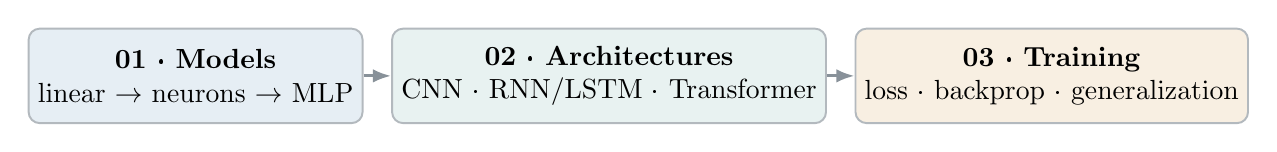
\begin{tikzpicture}[
    node distance=0.35cm,
    box/.style={rounded corners, minimum width=3.25cm, minimum height=1.2cm, align=center, draw=softink!35, line width=0.7pt},
    arrow/.style={-{Latex[length=2.3mm]}, line width=1.1pt, draw=softink!55}
  ]
    \node[box, fill=softblue!15] (intro) {\textbf{01 · Models}\\linear $\rightarrow$ neurons $\rightarrow$ MLP};
    \node[box, fill=softteal!15, right=of intro] (arch) {\textbf{02 · Architectures}\\CNN · RNN/LSTM · Transformer};
    \node[box, fill=softgold!18, right=of arch] (train) {\textbf{03 · Training}\\loss · backprop · generalization};
    \draw[arrow] (intro) -- (arch);
    \draw[arrow] (arch) -- (train);
  \end{tikzpicture}
  }
  \end{center}
  \vspace{0.4cm}
  \begin{itemize}
    \item This deck defines the models and their forward computation.
    \item Deck 02 asks how structure in images and sequences changes the architecture.
    \item Deck 03 explains how parameters are learned without contaminating the test set.
  \end{itemize}
\end{frame}

\sectiondivider{Learning from Data}

\begin{frame}{The Common Machine-Learning Pattern}
  \begin{center}
  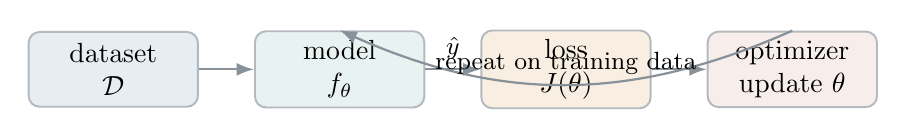
\begin{tikzpicture}[
    node distance=0.7cm,
    stage/.style={rounded corners, minimum width=2.15cm, minimum height=0.95cm, align=center, draw=softink!35, line width=0.7pt},
    arrow/.style={-{Latex[length=2.2mm]}, thick, draw=softink!55}
  ]
    \node[stage, fill=softblue!15] (data) {dataset\\$\mathcal D$};
    \node[stage, fill=softteal!15, right=of data] (model) {model\\$f_{\boldsymbol\theta}$};
    \node[stage, fill=softgold!18, right=of model] (loss) {loss\\$J(\boldsymbol\theta)$};
    \node[stage, fill=softcoral!14, right=of loss] (opt) {optimizer\\update $\boldsymbol\theta$};
    \draw[arrow] (data) -- (model);
    \draw[arrow] (model) -- node[above, font=\small] {$\hat y$} (loss);
    \draw[arrow] (loss) -- (opt);
    \draw[arrow, bend left=24] (opt.north) to node[above, font=\small] {repeat on training data} (model.north);
  \end{tikzpicture}
  \end{center}
  \begin{block}{One sentence}
    Choose parameters that make predictions accurate on training examples, while measuring whether the learned rule generalizes to unseen examples.
  \end{block}
\end{frame}

\begin{frame}{Examples, Features, and Targets}
  \[
    \mathcal D=\{(\mathbf x_i,y_i)\}_{i=1}^{n},
    \qquad \mathbf x_i\in\mathbb R^d
  \]
  \begin{columns}[T]
    \column{0.48\textwidth}
    \textcolor{softblue}{\textbf{Regression}}
    \begin{itemize}
      \item $y_i\in\mathbb R^m$
      \item predict displacement, temperature, demand
      \item output is numerical
    \end{itemize}
    \column{0.48\textwidth}
    \textcolor{softteal}{\textbf{Classification}}
    \begin{itemize}
      \item $y_i\in\{1,\ldots,C\}$
      \item predict material class or damage state
      \item output represents class probabilities
    \end{itemize}
  \end{columns}
  \vspace{0.25cm}
  \begin{alertblock}{Boundary rule}
    The labels, units, missing values, and admissible ranges are validated before model training.
  \end{alertblock}
\end{frame}

\begin{frame}{Train, Validate, Test}
  \begin{center}
  
\begin{tikzpicture}[
    part/.style={minimum height=1.05cm, draw=white, align=center, text=softink},
  ]
    \node[part, minimum width=6.2cm, fill=softblue!28] (train) {\textbf{training}\\fit parameters};
    \node[part, minimum width=3.2cm, fill=softgold!30, right=0pt of train] (val) {\textbf{validation}\\choose settings};
    \node[part, minimum width=2.4cm, fill=softteal!30, right=0pt of val] (test) {\textbf{test}\\final estimate};
  \end{tikzpicture}
  \end{center}
  \begin{itemize}
    \item Fit preprocessing statistics and model parameters using training data only.
    \item Use validation data for architecture, regularization, and early-stopping decisions.
    \item Evaluate the selected pipeline once on the untouched test set.
    \item Ratios depend on data volume and structure; time series and grouped samples need structure-aware splits.
  \end{itemize}
\end{frame}

\begin{frame}{Empirical Risk: One Objective, Many Models}
  \[
    \hat y_i=f_{\boldsymbol\theta}(\mathbf x_i),
    \qquad
    J(\boldsymbol\theta)=\frac{1}{n}\sum_{i=1}^{n}
    \ell(\hat y_i,y_i)
  \]
  \begin{itemize}
    \item $f_{\boldsymbol\theta}$: the chosen model family
    \item $\boldsymbol\theta$: all learnable weights and biases
    \item $\ell$: the error assigned to one example
    \item $J$: the mean training objective minimized by the optimizer
  \end{itemize}
  \begin{block}{Separation of responsibilities}
    The architecture defines possible predictions; the loss defines what counts as a good prediction; the optimizer searches for parameters.
  \end{block}
\end{frame}

\sectiondivider{Linear Models as Neurons}

\begin{frame}{Linear Regression Is an Affine Neuron}
  \begin{columns}[T]
    \column{0.52\textwidth}
    \[
      \hat y_i=\mathbf w^\top\mathbf x_i+b
    \]
    \[
      J(\mathbf w,b)=\frac{1}{2n}\sum_{i=1}^{n}(\hat y_i-y_i)^2
    \]
    \[
      \nabla_{\mathbf w}J=\frac1n\sum_i(\hat y_i-y_i)\mathbf x_i,
      \qquad
      \frac{\partial J}{\partial b}=\frac1n\sum_i(\hat y_i-y_i)
    \]
    \column{0.44\textwidth}
    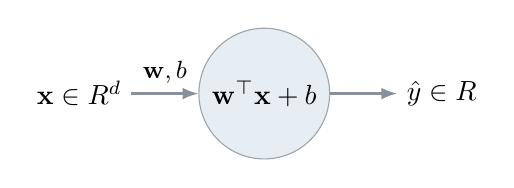
\begin{tikzpicture}[
      neuron/.style={circle, draw=softink!45, fill=softblue!15, minimum size=1.35cm},
      arrow/.style={-{Latex[length=2mm]}, thick, draw=softink!55}
    ]
      \node (x) {$\mathbf x\in\mathbb R^d$};
      \node[neuron, right=0.85cm of x] (n) {$\mathbf w^\top\mathbf x+b$};
      \node[right=0.85cm of n] (y) {$\hat y\in\mathbb R$};
      \draw[arrow] (x) -- node[above, font=\small] {$\mathbf w,b$} (n);
      \draw[arrow] (n) -- (y);
    \end{tikzpicture}
  \end{columns}
  \vspace{0.2cm}
  The factor $1/2$ is conventional: it cancels the $2$ produced by differentiating the square.
\end{frame}

\begin{frame}{Why a Linear Model Is Not Enough}
  \begin{figure}
    \centering
    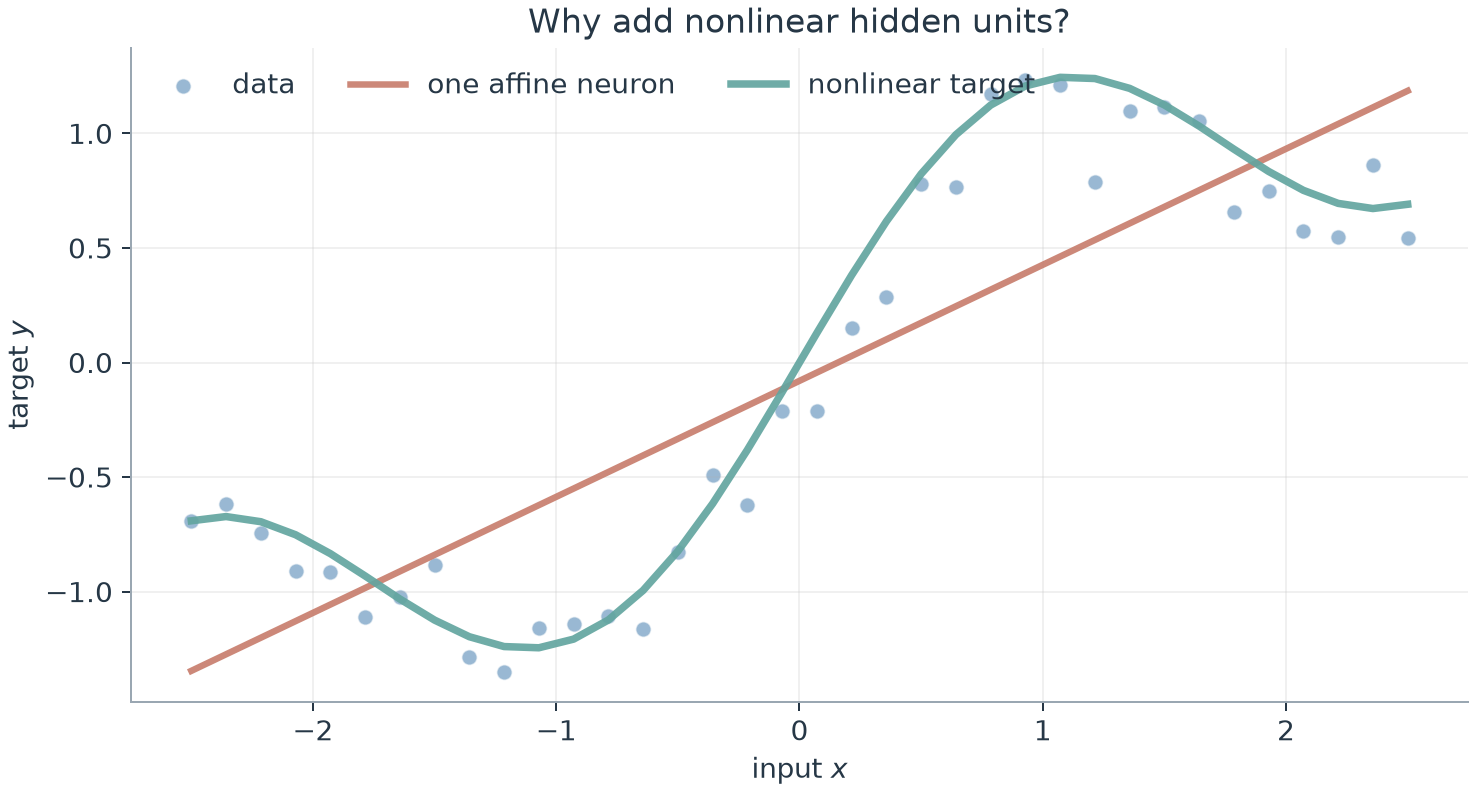
\includegraphics[width=0.72\linewidth]{regression_bridge.png}
  \end{figure}
  \vspace{-0.2cm}
  \begin{itemize}
    \item An affine model can tilt and shift a hyperplane, but it cannot bend it.
    \item Neural networks learn nonlinear intermediate features before the final prediction.
  \end{itemize}
\end{frame}

\begin{frame}{Logistic Regression Adds a Probabilistic Output}
  For binary labels $y_i\in\{0,1\}$:
  \[
    z_i=\mathbf w^\top\mathbf x_i+b,
    \qquad
    p_i=P(y_i=1\mid\mathbf x_i)=\sigma(z_i)=\frac{1}{1+e^{-z_i}}.
  \]
  Binary cross-entropy is the negative log-likelihood:
  \[
    J(\mathbf w,b)=-\frac1n\sum_{i=1}^{n}
    \left[y_i\log p_i+(1-y_i)\log(1-p_i)\right].
  \]
  Its gradient simplifies to
  \[
    \nabla_{\mathbf w}J=\frac1n\sum_i(p_i-y_i)\mathbf x_i,
    \qquad
    \frac{\partial J}{\partial b}=\frac1n\sum_i(p_i-y_i).
  \]
\end{frame}

\begin{frame}{A Neuron = Affine Map + Activation}
  \begin{center}
  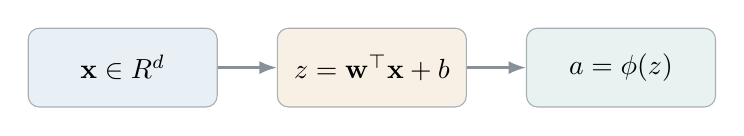
\begin{tikzpicture}[
    stage/.style={rounded corners, minimum width=2.4cm, minimum height=1.0cm, draw=softink!40, align=center},
    arrow/.style={-{Latex[length=2.2mm]}, thick, draw=softink!55},
    node distance=0.75cm
  ]
    \node[stage, fill=softblue!14] (input) {$\mathbf x\in\mathbb R^d$};
    \node[stage, fill=softgold!17, right=of input] (affine) {$z=\mathbf w^\top\mathbf x+b$};
    \node[stage, fill=softteal!15, right=of affine] (act) {$a=\phi(z)$};
    \draw[arrow] (input) -- (affine);
    \draw[arrow] (affine) -- (act);
  \end{tikzpicture}
  \end{center}
  \begin{itemize}
    \item The affine map mixes the input features.
    \item The activation makes the mapping nonlinear.
    \item Without nonlinear activations, any stack of affine layers collapses to one affine layer.
  \end{itemize}
\end{frame}

\begin{frame}{Common Hidden-Layer Activations}
  \begin{columns}
    \column{0.58\textwidth}
    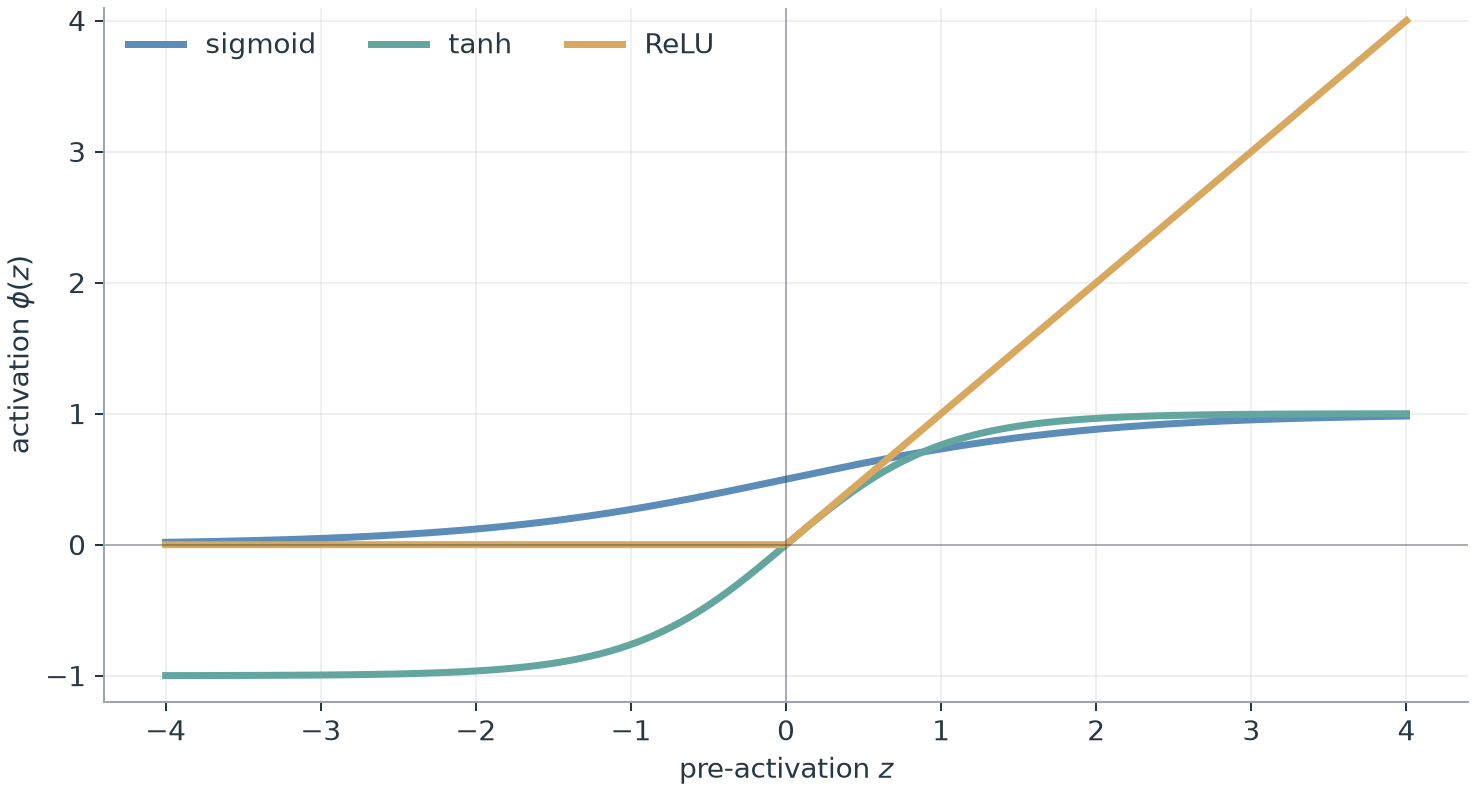
\includegraphics[width=\linewidth]{activation_functions.png}
    \column{0.39\textwidth}
    \small
    \textcolor{softgold}{\textbf{ReLU}}
    \[
      \phi(z)=\max(0,z)
    \]
    Common default in hidden layers.

    \medskip
    \textcolor{softteal}{\textbf{tanh}}
    Bounded and zero-centered; still useful in recurrent states.

    \medskip
    \textcolor{softblue}{\textbf{sigmoid}}
    Maps logits to $(0,1)$; useful for binary outputs and gates.
  \end{columns}
\end{frame}

\sectiondivider{Multilayer Perceptrons}

\begin{frame}{One Layer, With Dimensions}
  Let layer $\ell$ contain $d_\ell$ units. Then
  \[
    \mathbf a^{(0)}=\mathbf x\in\mathbb R^{d_0},
  \]
  \[
    \mathbf z^{(\ell)}
    =W^{(\ell)}\mathbf a^{(\ell-1)}+\mathbf b^{(\ell)},
    \qquad
    \mathbf a^{(\ell)}=\phi^{(\ell)}(\mathbf z^{(\ell)}),
  \]
  with
  \[
    W^{(\ell)}\in\mathbb R^{d_\ell\times d_{\ell-1}},
    \qquad
    \mathbf b^{(\ell)},\mathbf z^{(\ell)},\mathbf a^{(\ell)}\in\mathbb R^{d_\ell}.
  \]
  \begin{alertblock}{Shape check}
    The number of columns of $W^{(\ell)}$ must equal the number of outputs from layer $\ell-1$.
  \end{alertblock}
\end{frame}

\begin{frame}{A Multilayer Perceptron Composes Layers}
  \begin{center}
  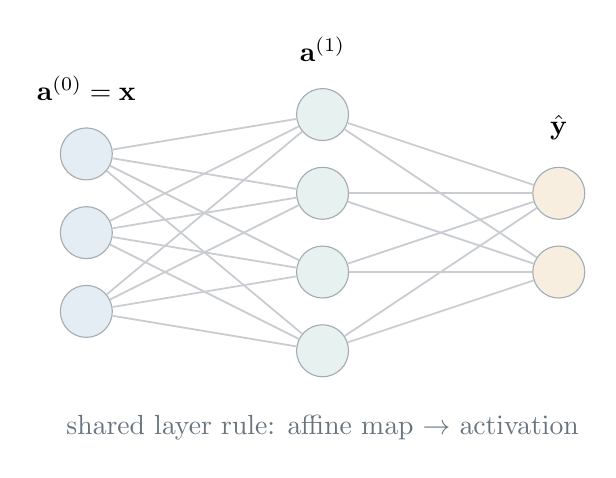
\begin{tikzpicture}[
    unit/.style={circle, draw=softink!42, minimum size=0.66cm},
    conn/.style={draw=softink!25, line width=0.65pt},
    >=Latex
  ]
    \foreach \y in {0,1,2} \node[unit, fill=softblue!16] (i\y) at (0,\y-1) {};
    \foreach \y in {0,1,2,3} \node[unit, fill=softteal!16] (h\y) at (3,\y-1.5) {};
    \foreach \y in {0,1} \node[unit, fill=softgold!20] (o\y) at (6,\y-0.5) {};
    \foreach \i in {0,1,2} \foreach \h in {0,1,2,3} \draw[conn] (i\i) -- (h\h);
    \foreach \h in {0,1,2,3} \foreach \o in {0,1} \draw[conn] (h\h) -- (o\o);
    \node[above] at (0,1.55) {$\mathbf a^{(0)}=\mathbf x$};
    \node[above] at (3,2.05) {$\mathbf a^{(1)}$};
    \node[above] at (6,1.05) {$\hat{\mathbf y}$};
    \node[below, text=softink!70] at (3,-2.2) {shared layer rule: affine map $\rightarrow$ activation};
  \end{tikzpicture}
  \end{center}
  \[
    f_{\boldsymbol\theta}(\mathbf x)
    =f^{(L)}\!\circ f^{(L-1)}\!\circ\cdots\circ f^{(1)}(\mathbf x)
  \]
\end{frame}

\begin{frame}{A Small Forward Pass}
  Let
  \[
    \mathbf x=\begin{bmatrix}2\\-1\end{bmatrix},\quad
    W^{(1)}=\begin{bmatrix}1&1\\-1&2\end{bmatrix},\quad
    \mathbf b^{(1)}=\begin{bmatrix}0\\1\end{bmatrix},\quad
    \phi=\operatorname{ReLU}.
  \]
  Hidden layer:
  \[
    \mathbf z^{(1)}=W^{(1)}\mathbf x+\mathbf b^{(1)}
    =\begin{bmatrix}1\\-3\end{bmatrix},
    \qquad
    \mathbf a^{(1)}=\begin{bmatrix}1\\0\end{bmatrix}.
  \]
  With $W^{(2)}=\begin{bmatrix}2&-1\end{bmatrix}$ and $b^{(2)}=0.5$:
  \[
    \hat y=W^{(2)}\mathbf a^{(1)}+b^{(2)}=2.5.
  \]
\end{frame}

\begin{frame}{The Output Layer Depends on the Task}
  \centering
  \begin{tabular}{lll}
    \toprule
    Task & Output & Typical loss \\
    \midrule
    Regression & $\hat{\mathbf y}=W\mathbf h+\mathbf b$ & mean squared error \\
    Binary classification & $p=\sigma(z)$ & binary cross-entropy \\
    $C$-class classification & $\mathbf p=\operatorname{softmax}(\mathbf z)$ & categorical cross-entropy \\
    \bottomrule
  \end{tabular}
  \vspace{0.45cm}
  \[
    p_c=\frac{e^{z_c}}{\sum_{j=1}^{C}e^{z_j}},
    \qquad
    \ell(\mathbf p,y)=-\log p_y.
  \]
  \begin{block}{Implementation note}
    Stable software computes cross-entropy directly from logits rather than taking the logarithm of rounded probabilities.
  \end{block}
\end{frame}

\begin{frame}{Takeaways}
  \begin{itemize}
    \item A learning problem combines data, a parametrized model, a loss, and an optimizer.
    \item Linear and logistic regression are single affine units with task-specific outputs.
    \item A neuron applies an affine map followed by an activation.
    \item An MLP composes these layers; dimensions make every operation checkable.
    \item Architecture determines the information-sharing pattern. That is the subject of Deck 02.
    \item Parameter learning, backpropagation, and generalization are deferred to Deck 03.
  \end{itemize}
\end{frame}

\end{document}
